\documentclass[conference]{IEEEtran}
\IEEEoverridecommandlockouts
% The preceding line is only needed to identify funding in the first footnote. If that is unneeded, please comment it out.
%Template version as of 6/27/2024

\usepackage{cite}
\usepackage{amsmath,amssymb,amsfonts}
\usepackage{algorithmic}
\usepackage{graphicx}
\usepackage{textcomp}
\usepackage{xcolor}

\usepackage{hyperref}

\def\BibTeX{{\rm B\kern-.05em{\sc i\kern-.025em b}\kern-.08em
    T\kern-.1667em\lower.7ex\hbox{E}\kern-.125emX}}
\begin{document}

\title{Classification and Clustering of Chess Portable Game Notation Text\\
%{\footnotesize \textsuperscript{*}}
%\thanks{Identify applicable funding agency here. If none, delete this.}
}

\author{\IEEEauthorblockN{Logan Miller}
\IEEEauthorblockA{\textit{Departments of Math and Computer Science}\\
\textit{Lawrence Technological University}\\
Southfield, MI, USA \\
lmiller2@ltu.edu}
\and
\IEEEauthorblockN{Rory Wilson}
\IEEEauthorblockA{\textit{Department of Math and Computer Science} \\
\textit{Lawrence Technological University}\\
Southfield, MI, USA \\
rwilson2@ltu.edu}
}

\maketitle

\begin{abstract}
This paper discusses using machine learning techniques on chess play analysis and players' skill levels, developing further from the inadequateness of traditional Elo-based metrics. By utilizing a dataset comprising several million chess games, this research applies k-means clustering to group games based on player ratings, move lengths, and their outcomes, revealing unique patterns across skill levels. It also uses Naive-Bayes classification to predict player Elo ratings from the moves and metadata of the games with striking accuracy.

These results really outline the power of incorporating diverse features with advanced methodologies for the extraction of deeper insights into player performance and gameplay dynamics. The key takeaways indicate that multi-feature clustering is effective for nuanced differences in the skill level and classification methods are useful in predicting performance. These advances open avenues for enhanced player training, personal feedback, and improvements in the chess engine. Future studies may add more features and symptom links and optimize different algorithms for better performance.
\end{abstract}

\begin{IEEEkeywords}
Machine Learning, Chess, Clustering Algorithms, Naive-Bayes Classification, Data Preprocessing, Skill Analysis, Player Performance Evaluation.
\end{IEEEkeywords}

\section{Introduction}
Chess is one of the oldest and most universally played strategy games, and with the advent of online platforms like chess.com, millions of games are now available for analysis. These platforms generate a wealth of data, which presents an opportunity to gain insights into player behavior, skill levels, and strategies. However, analyzing such large datasets to extract meaningful patterns remains a challenge. While traditional methods often focus on broad metrics like Elo ratings, they fail to account for the nuanced differences in play styles and strategies that define various skill levels. This paper aims to address this gap by employing machine learning techniques, specifically clustering and classification, to categorize chess games based on player skill levels and game play characteristics, offering a more granular understanding of player performance.

The importance of this problem lies in its potential to enhance player development, improve training tools, and refine chess engines. Automatically classifying games by skill level can provide valuable feedback to players, enabling personalized improvement suggestions. Additionally, it offers coaches and analysts a more detailed view of game play, which can inform training strategies. The key challenges in this task include handling the complex, high-dimensional nature of chess data and identifying relevant features that effectively differentiate skill levels. The two contributions of this work aim to attack the problem from both ends: The bottom-up approach is a novel clustering approach that groups games based on Elo ratings, move length, and game result, providing deeper insights into the relationship between game play and player expertise. The top-down approach is a direct analysis of the moves played in games via Naive-Bayes classification to correctly predict the Elo ratings of a player from their move lines.

\section{Related Work}
\subsection{Chess Text Clustering}
There have been more focused studies into chess text clustering. Such studies are  limitations such as testing on specific sets of opening moves \cite{b1}\cite{b2}. Our work is intended to encompass the whole of a game, including its ending, to determine similarity between games in the same skill level.
\subsection{Behavioral Clustering}
Using machine learning to identify player behavioral patterns is a well-trodden path. \cite{b3} is a meta-analysis on the topic, describing several reasonings for certain techniques to be used, with \cite{b7} and \cite{b8} showing various techniques in action, for already established games and those which are still growing, respectively. A chess-related extreme case is shown in \cite{b10}, in which the authors train models to identify players by their playstyle, including their mistakes.


\section{Methodology}
\subsection{Data Collection and Preprocessing}
Lichess.com is a popular online chess website where millions of games are played daily. These games are recorded and hosted at \href{https://database.lichess.org/}{database.lichess.org} under the Creative Commons CC0 license. We select the August 2015 selection of games to balance storage space with game selection: The Portable Game Notation format files uncompress to 7 times the file size, but there are over 2.6 million games across all skill levels to work with.

Portable Game Notation (PGN) is a format for the collection and storage of chess games in a manner that is easy to read for both computers and humans. \cite{b9} PGN text comes in the form of several tags, each a key-value pair enclosed within square brackets, and a list of moves in algebraic notation with a counter of how many full turns have passed. Since the text is already mainly of the form of key-value pairs, we read each one into a dictionary, with the moves coming after being added with the key "Moves."

%To gather the data about the different chess games there is a website https://database.lichess.org/ that is filled with different games with different levels of players. the data includes the move sequences, player ratings, game outcomes, and other metadata, which provides the foundation for clustering analysis. The data is cleaned by removing games with non-standard variants, incomplete results, or missing Elo ratings.
%
%Original data can be accessed under the open database at Lichess.org. This is a very good source of raw record data for chess games, such as several billion games within the Lichess platform. It maintains metadata about the players' ratings, time controls, and outcomes, along with full move sequences in PGN format. The database is a treasure for research due to its size, diversity, and good accessibility; material on most types of games and all skill levels from beginners through grandmasters is covered.

Not every game furnished in this file is appropriate for our purposes, however; Some may be variant games, some may not have the Elo rating of one or both players, or feature other such issues. We first check that each game is acceptable for our purposes by checking them against 4 criteria:
\begin{enumerate}
    \item The game must be a standard chess game (no variants).
    \item The game must have terminated normally (i.e. via checkmate).
    \item The game must have a normal result (1-0 White win, 0-1 Black win, 1/2-1/2 draw).
    \item The game must have valid Elo ratings for both players.
\end{enumerate}
If the game features meets all of these criteria, we include it in our dataset, and in total there are about 1.7 million suitable games in the dataset.

\begin{table}[htbp]
\vspace{.01cm}
\caption{Example Games from the Dataset}
\begin{center}
\begin{tabular}{|lllll|}
\hline
\multicolumn{5}{|c|}{lichess.org dataset}                                                                                                      \\ \hline
\multicolumn{1}{|l|}{White name}  & \multicolumn{1}{l|}{Black name} & \multicolumn{1}{l|}{Result} & \multicolumn{1}{l|}{White Elo} & Black Elo \\ \hline
\multicolumn{1}{|l|}{paul2chess3} & \multicolumn{1}{l|}{Andique}    & \multicolumn{1}{l|}{1-0}    & \multicolumn{1}{l|}{1509}      & 1623      \\ \hline
\multicolumn{1}{|l|}{Shenhewho}   & \multicolumn{1}{l|}{Gentux}     & \multicolumn{1}{l|}{1-0}    & \multicolumn{1}{l|}{1857}      & 1963      \\ \hline
\end{tabular}
\begin{minipage}{8cm}
    \vspace{0.1cm}
    \small The table above shows 2 games from the dataset showing the player names, the result of the game, and each player's Elo rating.
\end{minipage}
\end{center}
\label{table:example-games}
\end{table}

\subsection{Feature Extraction}

While a large amount of information is included in each PGN game, we only need a certain subset of data from each: The Elo ratings of the players, the result of the match-up, and the list of moves. While the Elo ratings and the result are their own tags and can be easily isolated, the moves require a bit of cleaning to be usable, removing all the turn counters, comments, and additional characters, as well as reducing whitespace. Deleting additional characters is important as it removes additional information like the exclamation points on brilliant moves and the question marks on blunders, to maintain the purity of the text.

As an additional angle to attempt, we use the chess-python library to also convert these PGN moves to moves in the format used by the Universal Chess Interface (UCI), which are only denoted by the square moved from concatenated with the square moved to, i.e. long algebraic notation without piece names as opposed to PGN's normal algebraic notation.

Every game is also condensed into a simple tuple of data to run additional measurements upon, consisting of just the White player's Elo rating, the length of the game in full moves, and the result of the game. This is documented in greater detail in Table \ref{table:example-games}, which outlines the structure and content of the files that make up the dataset.

For the purposes of measurement, Elo ratings are grouped into bins of width 100, with e.g. the 700s bin holding all games where the White player had an Elo rating between 700 and 799, inclusive. We record the number of games in each bin, as well as how many were wins, draws, or losses.

%this can be moved around to wherever
\begin{figure}[htbp]
\centerline{\includegraphics[scale=0.5]{Distribution and Win-Loss Proportion by Elo.png}}
\caption{Games Played vs. Elo Rating Bins (top): A bar chart showing the number of games played in each Elo rating range.
Win/Loss/Draw Proportions vs. Elo Rating (bottom): A stacked area chart visualizing the proportions of wins (green), losses (red), and draws (gray) for each Elo rating range.}
\label{fig:wl-prop}
\end{figure}

In terms of the distribution of games, it appears to closely follow a normal distribution (or a unimodal distribution of slight positive skew). Games in the range of 1400 to 1799 make up approximately 58\% of the dataset. There is a very clear positive correlation between Elo rating and win percentage, indicating that players with high Elo ratings win more of their games.

\subsection{Clustering Implementation}
 The cleaned dataset is used to group games based on player performance. The program applies the k-means clustering algorithm, leveraging Elo ratings as the primary axis for separation. Key steps include:
\begin{itemize}
    \item Determining the number of clusters (k): Using silhouette scores, the optimal value for k is selected, ensuring well-defined groupings.
    \item Running k-means: the algorithm partitions the data into clusters, where each cluster represents a subset of games with similar Elo ranges and gameplay characteristics.
\end{itemize}

K-means clustering does have some limitations as detailed in \cite{b4}, but the dataset used helps mitigate some of these: The density of the data is relatively dense within the 100-Elo bins, and the meticulous task of selecting a good value for k is greatly sped along via computation of silhouette score and examination of elbow curves.

After clustering the dataset, statistical analyses and visualization are performed to interpret the relationship between Elo ratings, game results, and gameplay patterns. these analyses highlight trends across different skill levels and provide actionable insight into the dataset.
\subsection{Classification Implementation}

Before attempting any sort of classification, we first remove the top and bottom 1\% of data for the purpose of removing any outliers.  Naive-Bayes text classification requires at least two distinct parts: The vectorizer, and the classifier. The choice of vectorizer and classifier can make a world of difference on the same dataset. In order to properly explore the space, we will use a variety of techniques and use every combination so that all possibilities are accounted for.

\section{Experimental Setup}

\subsection{Implementation Details}
Many different Python libraries were leveraged to work on this project:
\begin{itemize}
\item Numpy, for many quick implementations of mathematical operations.
\item Matplotlib, for all data visualizations.
\item Scikit-learn, for K-means implementation, Naive-Bayes classifications, and all related machine learning statistics.
\item python-chess, to convert all of the PGN data into acceptible UCI data.
\end{itemize}

For PGN elaboration, a custom parser has been used to extract relevant features from each suitable game: players' ratings, total moves, and the game's outcome. Then, data normalization was performed for correct clustering, while missing values were treated by deleting incomplete games. Therefore, k-means implementation was employed for the structured dataset, while the number of clusters was determined by the elbow method and silhouette score for the best performance. All the computations have been done on the free version of Google Colab, where computational resources were good enough to run this clustering analysis, though sometimes very limiting regarding duration and hardware.

\subsection{Evaluation Metrics}
Quality clustering for the PGN project was made using some different metrics; among them, the most important was the silhouette score since this score gives a measure of how well the clusters are kept apart, and how well the game fits within its assigned cluster. In that way, clusters reflect real differences in either the level of players or their style of play. Additionally, inertia (within-cluster sum of squares) was used to evaluate the compactness of data points within clusters. Cluster size distribution was analyzed to identify any imbalances or outliers affecting the clustering process. To ensure the clusters' interpretability, we compared results against logical groupings, such as player rating ranges or typical game lengths, confirming that the clusters provided insight into game dynamics. These also allow us to assess the performance of our approach against overall simpler baselines such as rating-only clustering.

\subsection{Baseline}
The baselines were necessary for giving a comparison to the effectiveness of the clustering methodology on PGN data. A simple baseline entails the grouping of chess games regarding players' ratings into pre-defined ranges of cut-off, for instance, beginning, intermediate, and advanced players. This was a simplified comparison that didn't give a deep scope on how other features such as game length and its outcome interact. Other baselines were k-means clustering on fewer features for further benchmark performance checks. Comparing those with our multi-feature clustering methodology, we could then illustrate the advantages of integrating diverse features for nuanced gameplay. Since we were on the free version of Google Colab, runtime and memory needed to be optimized for baseline testing to do efficient experiments within resource bounds.

\subsection{Hyperparameters}
The hyperparameters in this program are tuned carefully to optimize the clustering and feature extraction performance of the chess games. For the k-means clustering algorithm, the most important hyperparameter was the number of clusters derived from the unique groups of Elo rating determined by the program. This made sure that the grouping of the skill levels of players was logical. We varied the RESOLUTION parameter from this model to 500, which grouped the Elo ratings into bins of 500 (e.g. 0-499, 500-999, etc.), thus affecting clustering granularity. The preprocessing feature extraction also went through a TF-IDF vectorizer where, among its parameters, tokenization and stopword filtering were developed focusing on dealing with the densest pieces of text data. These hyperparameters control parsing data, such as GAME LIMIT, but also optional flags like DOUBLE GAMES. These balance the volume and variety of preprocessed data for scalability but still meaningful results. These have been iteratively tuned through testing to balance performance with computational efficiency.

\subsection{Classification}
We use a combination of a variety of classification techniques on both the PGN moves and the UCI moves to see which are best suited for the task. Each combination will be represented with a set of 3 symbols, to be appended to the document set used.
\begin{enumerate}
\item We compare and contrast two kinds of vectorizers. The first is a TF-IDF vectorization, with the idea being that players of a certain skill level will tend towards certain moves which can be used to distinguish them. The second is a vectorization to word counts as a baseline. It's important to make sure that the vectorizer does not force the text to lowercase; It doesn't matter with UCI, but PGN text has integral capitalization which needs to be preserved. This toggle is the first symbol of the set; TF-IDF vectorization will use \textbf{T} as its symbol, and word count vectorization will use \textbf{C}.
\item The data then needs to be split into a training group and a test group. 75\% of the data will be used to train the classifiers, and the remaining 25\% will be used to test their accuracy. The imbalance of the initial dataset is exaggerated with the increase in group size, so we additionally see how stratifying the data so that each class is equally represented affects the accuracy. If the data is stratified, the second symbol will be \textbf{1}, and if not, it will be \textbf{0}.
\item Two kinds of Naive-Bayes classifiers are used to attempt to model and predict the data. First is a Multinomial Naive-Bayes (MNB) classification, and the second is a Complement Naive-Bayes (CNB) classification. CNB is designed to take the complement of each class for its weights, and is suited to imbalanced datasets. Theoretically, CMB will perform better than MNB due to the imbalance of the dataset it will be given. MNB will be \textbf{M}, CMB will be \textbf{C}.
\end{enumerate}

As an example, UCI text which is treated to a TF-IDF vectorization, stratified data, and Complement Naive-Bayes classification will be represented as "UCI-T1C."

%\subsection{Figures and Tables}\label{}
%\paragraph{Positioning Figures and Tables} Place figures and tables at the top and 
%bottom of columns. Avoid placing them in the middle of columns. Large 
%figures and tables may span across both columns. Figure captions should be 
%bElow the figures; table heads should appear above the tables. Insert 
%figures and tables after they are cited in the text. Use the abbreviation 
%``Fig.~\ref{fig}'', even at the beginning of a sentence.

\section{Results and Discussion}

\subsection{Clustering}

\begin{figure}[htbp]
\centerline{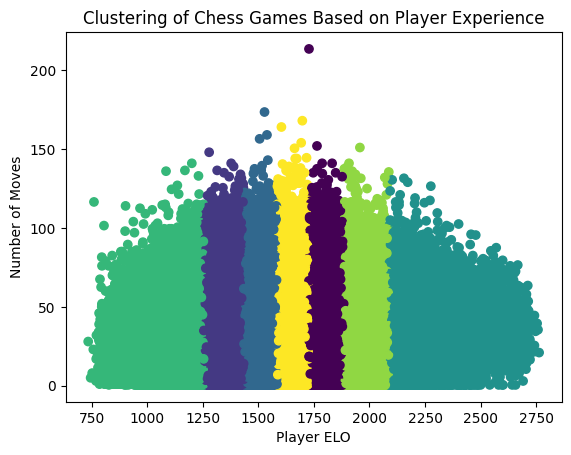
\includegraphics[scale=0.5]{Clustering of Chess Games Based on Experience.png}}
\label{fig:cluster-results}
\caption{A scatterplot of all the games in consideration, colored in accordance to which cluster they belong to.}
\end{figure}

Using k=7 clusters, all the games quickly and cleanly separate out into nearly-equal width bands between 1250 Elo and about 2100 Elo. Any values below 1250 are in their own cluster, and any values above 2100 are in their own cluster as well. Interestingly, this seems to remain true even when the cluster count increases, with the bands in between getting thinner to fit. This isn't an intentional feature of the clustering algorithm, but it's one that works in our advantage: These self-inforced bounds are roughly equivalent to the bound between novices and intermediate players, and the bound between intermediate players and experts \cite{b6}. Move length seems to have no bearing on the clustering at all.

\subsection{Classification}
\begin{table}[htbp]
\caption{Classification Accuracy by Method Group}
\centering
\begin{tabular}{lr}
\hline\hline
Method Group & Accuracy \\ [0.5ex]
\hline
PGN-T1M & 62.232\% \\
PGN-T1C & 55.506\% \\
PGN-T0M & \textbf{62.265\%} \\
PGN-T0C & 55.521\% \\
PGN-C1M & 57.756\% \\
PGN-C1C & 55.038\% \\
PGN-C0M & 57.753\% \\
PGN-C0C & 55.062\% \\ [1ex]
\hline
\end{tabular}
\begin{tabular}{lr}
\hline\hline
Method Group & Accuracy \\ [0.5ex]
\hline
UCI-T1M & 62.297\% \\
UCI-T1C & 55.599\% \\
UCI-T0M & \textbf{62.330\%} \\
UCI-T0C & 55.623\% \\
UCI-C1M & 56.749\% \\
UCI-C1C & 54.837\% \\
UCI-C0M & 56.741\% \\
UCI-C0C & 54.787\% \\ [1ex]
\hline
\end{tabular}
\label{table:class-results}
\end{table}

Table \ref{table:class-results} contains the accuracy scores of each of the 8 combinations of classification techniques for both document sets. On PGN text, the highest accuracy is 62.265\%, with the Multinomial Naive-Bayes classifier, unstratified data splits, and the TF-IDF vectorizer (PGN-T0M). These same settings produce the highest accuracy for UCI text as well, at 62.330\% (UCI-T0M).

Some trends appear in regards to how specific choices affect the average accuracy of the predictions.
\begin{itemize}
\item Generally, classification is improved by using TF-IDF vectorization over word count vectorization, with MNB losing approximately 5-6\% accuracy when switching between the two and CMB losing 0.5-0.9\%.
\item Strafitication affected accuracy very little, with the random sampling picking approximately the same frequency of classes as the guaranteed frequencies enforced by stratification. In most cases, not using stratification increased overall accuracy by a few hundredths of a percentage point, except when using UCI text with word count vectorization, in which case accuracy decreases approximately 0.008\% with MNB and 0.05\% with CMB.
\item Against expectations, Multinomial Naive-Bayes outperforms Complement Naive-Bayes in all cases, being approximately 7\% more accurate with TD-IDF vectorization and 2\% more accurate with word count vectorization.
\end{itemize}

\section{Conclusion}

It should be done in a way to show the power of machine learning techniques in analyzing games and a player's skill in chess. This project uses k-means clustering and Naive-Bayes classification to address some issues with traditional Elo-based analyses and provides comprehensive information on player performance and game dynamics.

\begin{itemize}
    \item  A multifeature clustering that groups games based on player ratings, move lengths, and outcome indeed reflects different patterns for different skill levels.
    \item Classification methods using game move and metadata inputs capable of accurately predicting player Elo ratings.
\end{itemize}

The results also show the importance of incorporating various features and state-of-the-art methods to find deeper trends within chess data. These techniques will lead to better training of players, provide personal feedback, and help developers improve their chess engines. Further works can be done by incorporating other features or optimizing algorithms to achieve higher accuracy and computational efficiency.

%Figure Labels: Use 8 point Times New Roman for Figure labels. Use words 
%rather than symbols or abbreviations when writing Figure axis labels to 
%avoid confusing the reader. As an example, write the quantity 
%``Magnetization'', or ``Magnetization, M'', not just ``M''. If including 
%units in the label, present them within parentheses. Do not label axes only 
%with units. In the example, write ``Magnetization (A/m)'' or ``Magnetization 
%\{A[m(1)]\}'', not just ``A/m''. Do not label axes with a ratio of 
%quantities and units. For example, write ``Temperature (K)'', not 
%``Temperature/K''.

\begin{thebibliography}{00}
\bibitem{b1} F. Wijayanto, “Clustering Analysis of Chess Portable Game Notation Text,” Jurnal Sains, Nalar, Dan Aplikasi Teknologi Informasi, vol. 3, no. 3, pp. 137–142, 2024.
\bibitem{b2}K. Raghav and L. Ahuja, “Chess Opening Analysis Using DBSCAN Clustering and Predictive Modeling,” in 2024 11th International Conference on Reliability, Infocom Technologies and Optimization (Trends and Future Directions) (ICRITO), Noida, India, Mar. 14–15, 2024, pp. 1–5.
\bibitem{b3} C. Bauckhage, A. Drachen, and R. Sifa, “Clustering Game Behavior Data,” IEEE Transactions on Computational Intelligence and AI in Games, vol. 7, no. 3, 2015.
\bibitem{b4} S. Shukla and S. Naganna, “A review on K-means data clustering approach,” International Journal of Information \& Computation Technology, vol. 4, no. 17, pp. 1847–1860, 2014.
\bibitem{b5} T. Kanungo, D. M. Mount, N. S. Netanyahu, C. D. Piatko, R. Silverman, and A. Y. Wu, “An efficient K-means clustering algorithm: Analysis and implementation,” IEEE Transactions on Pattern Analysis and Machine Intelligence, vol. 24, no. 7, pp., 2002.
\bibitem{b6} A. Elo, "The Rating of Chess Players, Past and Present," 1978 via gwern.net, https://gwern.net/doc/statistics/order/comparison/1978-elo-theratingofchessplayerspastandpresent.pdf, p.6.
\bibitem{b7} D. Shamsudin, L. M. Chew, and O. L. Yeng, “Clustering algorithms analysis based on arcade game player behavior,” in 2022 IEEE Fifth International Conference on Artificial Intelligence and Knowledge Engineering (AIKE), Laguna Hills, CA, USA, Sept. 19–21, 2022, pp. 122–125.
\bibitem{b8} H. Kwon, W. Jeong, D.-W. Kim, and S.-I. Yang, “Clustering player behavioral data and improving performance of churn prediction from mobile game,” in 2018 International Conference on Information and Communication Technology Convergence (ICTC), Jeju Island, Korea (South), Oct. 17–19, 2018, pp. 1252–1254.
\bibitem{b9} S. Edwards, "PGN Standard," March 12, 1994 via Internet Archive, https://archive.org/details/pgn-standard-1994-03-12
\bibitem{b10} R. McIlroy-Young, R. wang, S. Sen, J. Kleinberg, and A. Anderson, "Learning models of individual behavior in chess," in Proceedings of the 28th ACM SIGKDD Conference on Knowledge Discovery and Data Mining, 2022, pp.. 1253-1265.
\end{thebibliography}

\end{document}
